% !TEX program = xelatex
% VERSÃO REVISADA do artigo v2 (26/11/2026), com as sugestões de revisão: Eq. (9) numa base de volume só; turbina com o
% rendimento do modelo orçado (31,5%, Taurus 60); troca das pilhas e encargos da FV no caso-base e no Monte Carlo;
% validação e disponibilidade do modelo; contribuição frente a Castiñeiras-Filho et al. (2025); análise exergética.
% Números: caso_rev.js, incerteza_rev.js e otimiza_rev.js (motor modelo_rev.js); figuras: figs/gera_figs_rev.py.
% Compilar: python artigo_v2/monta_rev.py   (ou xelatex Grupo-03__Artigo_rev.tex, depois de gerar refs_ordenadas_rev.tex)
% O original (Grupo-03__Artigo.tex) não foi alterado. Revisão final: revisao_final_patch.py, _patch2.py, _patch3.py, _patch4.py (tarifa TG1) e _patch5.py.
\documentclass[10pt,a4paper,twocolumn]{article}
\frenchspacing
\usepackage[a4paper,top=24mm,bottom=24mm,left=15mm,right=15mm,columnsep=6mm,footskip=10mm]{geometry}
\usepackage{fontspec}
\usepackage[brazilian,provide=*]{babel} % provide=*: carrega o português pelo .ini do babel, sem depender do pacote babel-portuges
\usepackage{amsmath}
\usepackage{unicode-math}
\setmainfont{texgyretermes}[Extension=.otf,UprightFont=*-regular,BoldFont=*-bold,ItalicFont=*-italic,BoldItalicFont=*-bolditalic]
\setmathfont{texgyretermes-math.otf}
\usepackage{microtype}
\usepackage{graphicx}
\usepackage{booktabs,array}
\usepackage[font=normalsize,labelsep=period,justification=centering,skip=4pt]{caption}
\captionsetup[figure]{name=Fig.}
\captionsetup[table]{name=Tabela,position=top}
\usepackage{titlesec}
\usepackage{enumitem}
\usepackage{xurl}
\usepackage[hidelinks]{hyperref}

\titleformat{\section}{\normalfont\normalsize\bfseries}{\thesection.}{0.5em}{}
\titlespacing*{\section}{0pt}{9pt}{4pt}
\titleformat{\subsection}{\normalfont\normalsize\itshape}{\thesubsection.}{0.5em}{}
\titlespacing*{\subsection}{0pt}{6pt}{3pt}
\setlength{\parindent}{3.5mm}
\setlength{\parskip}{0pt}
\setlist{nosep,leftmargin=4mm}
\renewcommand{\arraystretch}{1.12}
\setlength{\tabcolsep}{3.2pt}
\setlength{\abovedisplayskip}{4pt}\setlength{\belowdisplayskip}{4pt}
\setlength{\abovedisplayshortskip}{2pt}\setlength{\belowdisplayshortskip}{3pt}
\setlength{\textfloatsep}{8pt plus 2pt}\setlength{\floatsep}{8pt plus 2pt}\setlength{\dbltextfloatsep}{8pt plus 2pt}
\renewcommand{\topfraction}{0.9}\renewcommand{\bottomfraction}{0.6}\renewcommand{\textfraction}{0.08}
\renewcommand{\dbltopfraction}{0.9}\renewcommand{\floatpagefraction}{0.8}\renewcommand{\dblfloatpagefraction}{0.8}
\newcolumntype{L}[1]{>{\raggedright\arraybackslash}p{#1}}
\newcommand{\MJt}{MJ\textsubscript{t}}
\newcommand{\MJe}{MJ\textsubscript{e}}
\newcommand{\Ht}{H\textsubscript{2}}
\newcommand{\Ot}{O\textsubscript{2}}
\newcommand{\COt}{CO\textsubscript{2}}
\newcommand{\un}[1]{\,\mathrm{#1}}
\pagestyle{plain}

\begin{document}
\twocolumn[{%
\begin{center}
{\fontsize{24}{27}\selectfont Descarbonização da fabricação de porcelanato com hidrogênio e recuperação de calor: balanços de energia e exergia, incerteza e avaliação econômica\par}
\vspace{10pt}
{\fontsize{12}{14}\selectfont Eduardo Alves Batista Vaz*\textsuperscript{‡}, Matheus Rodrigues da Costa*, Vinicius dos Santos Florenzano*\par}
\vspace{6pt}
*Curso de Engenharia de Energia, Universidade Federal de Itajubá (UNIFEI), Av. BPS, 1303, 37500-903, Itajubá, MG, Brasil\par
(eduardoab.vaz@gmail.com)\par
\vspace{4pt}
\textsuperscript{‡} Autor correspondente; Eduardo Alves Batista Vaz, Av. BPS, 1303, Itajubá, MG, Brasil, eduardoab.vaz@gmail.com\par
\vspace{4pt}
Recebido: xx.xx.xxxx Aceito: xx.xx.xxxx\par
\end{center}
\vspace{2pt}
\noindent\rule{\textwidth}{0.4pt}\par\vspace{3pt}
\noindent\textbf{Resumo-} Na fabricação de porcelanato por via úmida, quase toda a energia vai para atomização, secagem e queima, supridas por gás natural. Este trabalho quantifica, \textit{gate-to-gate} e por m² de produto (22,00~kg), os balanços de massa, energia e exergia de uma indústria de referência de 30.000~m²/dia em Santa Catarina, o efeito da recuperação de calor do forno e um ciclo com hidrogênio de eletrólise suprida por um campo fotovoltaico dedicado, ligado à rede. A referência consome 119,99~MJ/m² e emite 6,08~kg/m² de \COt; recuperar calor do forno reduz as emissões em 19\% e eleva a eficiência exergética de 31\% para 37\%. No ciclo proposto, uma turbina a gás com 30\% de \Ht{} em volume e o rendimento de catálogo do modelo orçado (31,5\%) gera a eletricidade da planta, seu escape aquece o atomizador e o forno queima \Ht{} com o oxigênio da eletrólise: as emissões caem 61\%, para 2,39~kg/m², mas a eficiência exergética, numa fronteira ampliada que inclui a eletricidade do campo fotovoltaico, cai para 25\%: a rede e o eletrolisador destroem 50,7~MJ/m² e a turbina, 21,0. Com todos os custos orçados, inclusive a troca das pilhas e os encargos da fotovoltaica, o investimento é de US\$~262,8 milhões, o valor presente líquido a 8\% ao ano em 25 anos é de −US\$~242,4 milhões, o \Ht{} custa US\$~6,58/kg e evitar \COt{} custa US\$~562/t. Num Monte Carlo com dez hipóteses sorteadas juntas, nenhuma combinação se paga com o gás de hoje, e o gás teria de passar de R\$~10,99/m³ para o projeto se pagar com 90\% de probabilidade. O modelo, o código e a semente estão disponíveis.\par
\vspace{3pt}
\noindent\textbf{Palavras-chave} porcelanato; recuperação de calor; hidrogênio; exergia; incerteza; avaliação econômica.\par
\noindent\rule{\textwidth}{0.4pt}\par\vspace{8pt}
}]

\section{Introdução}

O porcelanato é um revestimento cerâmico de baixíssima absorção de água, produzido no Brasil predominantemente por via úmida: as matérias-primas são moídas com água, a suspensão (barbotina) é seca por atomização, o pó é prensado, seco, esmaltado e queimado em forno a rolos a cerca de 1.200~°C \cite{oliveira2015}. Atomização, secagem e queima concentram a maior parte da energia, quase toda suprida por gás natural \cite{mctic2017,monfort2010}. A descarbonização depende, portanto, tanto do aproveitamento do calor hoje descartado quanto da troca do combustível.

Para a indústria cerâmica brasileira, Castiñeiras-Filho \textit{et al.} \cite{castineiras2025} avaliaram a substituição de 15\% do gás natural dos secadores de uma fábrica de Rio Claro (SP) por \Ht{} de um eletrolisador de 2,5~MW, com eletricidade a R\$~300/MWh: o \Ht{} custou de US\$~2,84/kg, com o \Ot{} valorizado na combustão enriquecida, a US\$~5,56/kg, e o projeto se pagaria com o gás acima de R\$~8,55/m³. O estudo usa cenários determinísticos e sensibilidades de uma ou duas variáveis, sem recuperação de calor, sem incerteza conjunta e sem análise exergética. Do lado termodinâmico, Ferrer \textit{et al.} \cite{ferrer2019} e Wang, Yang e Xu \cite{wang2020} fizeram balanços de exergia de fornos a rolos industriais e atribuíram a maior parte da exergia destruída à combustão e à troca de calor, mas sem trocar o combustível nem integrar o forno ao restante da fábrica.

Este artigo resume o Projeto II do Grupo 3 da disciplina EEN807 da UNIFEI e acrescenta a esses trabalhos três contribuições. (i) \textit{Integração:} numa mesma fronteira \textit{gate-to-gate}, com balanços fechados por m², tratam-se juntos a recuperação do calor do forno, uma turbina a gás com 30\% de \Ht{} cujo escape alimenta o atomizador e o forno a \Ht{} com o \Ot{} da eletrólise, e a análise exergética mostra onde cada escolha de integração destrói ou poupa exergia. (ii) \textit{Condições brasileiras:} o custo de cada equipamento e o fluxo de caixa incluem câmbio, importação, tarifas de uso da rede, acerto na Câmara de Comercialização de Energia Elétrica (CCEE), encargos da fotovoltaica e o limite de conciliação do Sistema Brasileiro de Comércio de Emissões (SBCE). (iii) \textit{Incerteza com otimização:} o mesmo modelo, verificado contra a planilha de precificação, é usado num Monte Carlo e na otimização do tamanho do eletrolisador e do uso do \Ht, com código e semente disponíveis. A indústria de referência, aqui chamada de ciclo 0, é uma base de cálculo (só gás natural e eletricidade da rede, sem recuperação de calor), e não a unidade de Tijucas, que forneceu os dados.

\section{Processo, dados e método}

\subsection{Escopo e unidade funcional}

A fronteira é \textit{gate-to-gate}, do recebimento das matérias-primas à expedição, em doze etapas: recepção, dosagem, moagem a úmido, peneiramento, atomização, repouso, prensagem, secagem, esmaltação, queima, retífica e expedição. A unidade funcional é 1~m² de porcelanato acabado com 22,00~kg \cite{alves2023a}; a escala de 30.000~m²/dia (10,95 milhões de m²/ano) converte os valores por m² em potências, vazões e custos. Por restrição do projeto, a fotovoltaica só aparece como sistema à parte, dedicado ao eletrolisador e fora do balanço da planta. Energia térmica é indicada em \MJt{} e elétrica em \MJe, ambas por m², com $1\un{kWh}=3{,}6\un{MJ}$; os combustíveis são contabilizados pelo poder calorífico inferior (PCI) e as correntes gasosas pelo calor sensível acima de 25~°C. Todos os volumes de gás, do gás natural e do \Ht, estão em m³ a 20~°C e 1~atm, a base em que a distribuidora cobra o gás. As contas foram feitas sem arredondar; algumas somas diferem na última casa.

\subsection{Base de dados}\label{sec:dados}

Os dados de planta vêm da unidade da Portobello em Tijucas (SC). Do relatório de sustentabilidade vêm o consumo específico consolidado de 0,12~GJ/m² (p. 51), a captação de água de 12,16 L/m² (p. 56) e a conferência da fração térmica de 88\% (de 2023 a 2025, o gás natural foi de 86,6\% a 88,3\% da soma de gás e eletricidade; p. 109 e 110, calculado pelo grupo) \cite{portobello2025}. Por comunicação técnica, cedidos para uso acadêmico, vêm o consumo do moinho contínuo (cerca do dobro dos 36 a 43~kWh/t de \cite{alves2023b}; adotados 80~kWh/t), o reaproveitamento do ar de resfriamento e as faixas de queima, atomização e secagem, 49\% a 55\%, 36\% a 39\% e 9\% a 12\% da demanda térmica, consideradas realistas \cite{rigobelo2026}; adotou-se o meio delas, 52,0\%, 37,5\% e 10,5\% (o MCTIC dá 49\%, 39\% e 12\% \cite{mctic2017}). O ciclo 0 toma o consumo consolidado de Tijucas (hipótese), mas não o seu reaproveitamento; os resultados valem para essa indústria de referência. Os demais parâmetros vêm da literatura ou são hipóteses (Tabela~\ref{tab:premissas}). O PCI do gás natural, 35,9~MJ/m³ a 20~°C e 1~atm, é hipótese do grupo, entre os 35,5~MJ/m³ do poder calorífico de referência da SCGÁS \cite{scgas2026}, convertido pela razão PCI/PCS do metano \cite{cengel2013}, e os 36,8~MJ/m³ da média nacional de 2025 \cite{anp2026}; nos dois extremos, os volumes mudariam de −2,4\% a +1,1\%, e o balanço e o \COt, feitos em MJ, não mudam.

\begin{table}[!t]
\centering
\caption{Principais premissas}\label{tab:premissas}
\footnotesize
\begin{tabular}{L{3.85cm}L{2.05cm}L{1.95cm}}
\toprule
\textbf{Parâmetro} & \textbf{Valor} & \textbf{Origem}\\ \midrule
Massa do produto & 22,00~kg/m² & \cite{alves2023a}\\
Umidade: barbotina / pó / seco & 33,8 / 6,0 / 0,3\% & \cite{oliveira2015,negre2000}\\
Umidade das matérias-primas & 4\% (na região, até 22\% \cite{rigobelo2026}) & hipótese\\
Esmalte: suspensão / sólidos & 1,10~kg/m² / 70\% & hipótese\\
Perda ao fogo na queima & 0,97~kg/m² & hipótese; realista em \cite{rigobelo2026}\\
Lama de retífica & 0,78~kg/m² & hipótese; ordem de \cite{sartor2021}\\
Consumo específico & 33,33~kWh/m² & \cite{portobello2025}, p. 51 (hipótese: o da referência)\\
Fração térmica do consumo & 88\% & adotada; conferida com \cite{portobello2025}\\
Queima / atomização / secagem & 52,0 / 37,5 / 10,5\% & meio das faixas realistas em \cite{rigobelo2026}\\
Gás do forno: exaustão / ar de resfriamento & 51,3 / 27,8\% & \cite{brown1996}\\
PCI: \Ht{} / gás natural & 120,0~MJ/kg / 35,9~MJ/m³ & \cite{cengel2013} / hipótese\\
$c_p$: ar e exaustão / escape / gás de combustão / vapor & 1,05 / 1,10 / 1,07 / 1,90 kJ/(kg·K) & estimados de \cite{cengel2013}\\
Temperatura: exaustão / ar de resfriamento do forno & 200 / 225~°C & hipótese\\
Temperatura: exaustão na saída do trocador / ar aquecido & 140 / 150~°C & hipótese (140~°C: orvalho ácido)\\
Pressão: eletrolisador / estoque de \Ht{} / turbina / queimadores / estoque de \Ot & 30 / 200 / 25 / 0,25 / 30~bar & hipótese\\
Fator de emissão: gás natural / sistema interligado & 56,1~kg/GJ / 0,0385~kg/kWh & \cite{ipcc2006} / \cite{mcti2024}\\
Excesso de ar no forno a gás ($\lambda$) & 1,15 & hipótese\\
Recuperação do ar de resfriamento / rendimento do trocador & 85 / 85\% & hipótese\\
Eletricidade dos ventiladores da recuperação & 0,60~\MJe/m² & hipótese (estimativa)\\
Entrada do atomizador & 550~°C & \cite{della2012}\\
Rendimento elétrico da turbina & 31,5\% & catálogo do Taurus 60 \cite{gtw2018,solar2026}\\
Escape da turbina & 500~°C & \cite{boyce2012}\\
\Ht{} na mistura da turbina & 30\% vol. & \cite{netl2022}\\
Consumo do eletrolisador & 58~kWh/kg & de \cite{iea2025b} (57,5) + compressão (hipótese)\\
Pilha: custo / vida & 17,5\% do eletrolisador / 50.000~h & \cite{iea2025a} (15--20\%) / \cite{iea2025b}\\
Encargos da fotovoltaica & R\$~120/(kW·ano) & \cite{epe2025}\\
Produtividade da FV (leste-oeste) & 1.137,5~kWh/\allowbreak{}(kWp·ano) & adotada de \cite{canalsolar2022,pvmag2021}\\
Estado morto (exergia) & 25~°C e 1~atm & hipótese\\
Exergia química: CH\textsubscript{4} / \Ht{} / \Ot & 831,65 / 236,09 / 3,97~kJ/mol & \cite{bejan1996}\\
Exergia retida na peça & 10\% da entrada do forno a gás & \cite{ferrer2019}\\
Gases de secagem no secador & 125~°C & \cite{mezquita2012}\\
\bottomrule
\end{tabular}
\end{table}

\subsection{Balanço de massa}

Como a massa de sólidos secos $m_s$ se conserva nas secagens, a massa de uma corrente com umidade $x$ em base úmida é
\begin{equation}
m = \frac{m_s}{1-x}. \label{eq:mtotal}
\end{equation}
Resolvido do produto para trás, o balanço dá 24,06~kg/m² de matéria-prima, 34,72 de barbotina, 24,45 de pó, 23,05 de peça seca, 24,15 de peça esmaltada e 22,78 de peça queimada. Entram 35,94~kg/m² (matéria-prima, 10,78 de água de moagem e 1,10 de suspensão de esmalte) e saem 35,94: 22,00 de produto, 12,07 de água evaporada (10,27 no atomizador, 1,40 no secador e 0,40 no forno), 0,97 de perda ao fogo, 0,78 de lama de retífica e 0,12 de perda de manuseio (0,5\%, hipótese).

\subsection{Modelo, verificação e validação}\label{sec:modelo}

Todas as contas saem de um modelo único: 179 grandezas técnicas, cada uma com fórmula, unidade e fonte, avaliadas em ordem de dependência, e um modelo econômico que segue a planilha de precificação item a item. O mesmo código alimenta o memorial, o site do projeto, a sensibilidade, o Monte Carlo, a otimização e a análise exergética. Foram feitas quatro verificações: (1) os balanços de massa, energia e exergia fecham (as diferenças são de arredondamento, abaixo de 0,02~MJ/m²); (2) com as hipóteses da versão anterior, o código reproduz o VPL da planilha com diferença de US\$~0,05 milhão; (3) o Monte Carlo, repetido com outra semente, muda no máximo 0,51\% em qualquer percentil da Tabela~\ref{tab:mc_sai}; (4) a otimização reproduz o caso-base nos dois métodos (Seção~\ref{sec:otim}).

Não há dados medidos por operação da planta (não são públicos); por isso a validação compara indicadores que o modelo \textit{calcula} com valores publicados que ele \textit{não usa} (Tabela~\ref{tab:valid}). Os consumos específicos e o calor do forno ficam nas faixas da literatura; a moagem fica acima, o que é coerente com o moinho contínuo de Tijucas \cite{rigobelo2026}. A água evaporada só confere a ordem de grandeza, porque a umidade das matérias-primas não passa pela captação. A exergia destruída no forno a gás (73\% da entrada, com as perdas pelas paredes) fica abaixo dos 83\% e 85\% medidos em fornos a rolos \cite{ferrer2019,wang2020}, porque a repartição de Brown \textit{et al.} \cite{brown1996} põe mais calor nas chaminés, onde ele é perda, e não destruição. O \Ht{} e o gás que zera o VPL ficam acima dos de \cite{castineiras2025}, que usa eletricidade a R\$~300/MWh, 15\% de substituição e vida de 20 anos a 5\% ao ano; a ordem de grandeza é a mesma.

\begin{table}[!t]
\centering
\caption{Validação: indicadores calculados pelo modelo e valores publicados que ele não usa}\label{tab:valid}
\footnotesize
\begin{tabular}{L{3.3cm}rL{2.4cm}}
\toprule
\textbf{Indicador} & \textbf{Modelo} & \textbf{Referência}\\ \midrule
Calor do ciclo 0 (GJ/t de produto) & 4,80 & 3,5--5,0 \cite{monfort2010}\\
Forno (MJ/kg de produto) & 2,50 & 2,0--2,8 \cite{monfort2010}\\
Forno (kcal/kg de produto) & 596 & 500--600 \cite[p.~115]{oliveira2015}\\
Atomizador (MJ/kg de água) & 3,86 & 3,8--4,6 \cite{negre2000}\\
Eletricidade (kWh/t de produto) & 182 & 138--192 \cite{monfort2010}\\
Moagem (kWh/t de sólido seco) & 83,8 & 52 ± 15 \cite{monfort2010}\\
Água evaporada (kg/m²) & 12,07 & captação de 12,16 L/m² \cite{portobello2025}\\
Calor do forno nas chaminés e no ar & 79\% & mais de 60\% nas chaminés \cite{ferrer2019}\\
Exergia destruída no forno a gás & 73\% & 83\% \cite{ferrer2019}; 85\% \cite{wang2020}\\
Eletrolisador (kWh/kg) & 58 & 61,7 \cite{castineiras2025}\\
Custo do \Ht{} (US\$/kg) & 6,58 & 2,84--5,56 \cite{castineiras2025}\\
Gás que zera o VPL (R\$/m³) & 9,80 & 8,55 \cite{castineiras2025}\\
\bottomrule
\end{tabular}
\end{table}

\section{Ciclo 0: energia e emissões}

O consumo consolidado de 33,33~kWh/m² se divide em
\begin{align}
Q_{t,0} &= f_t\, E_{\text{tot}} = 0{,}88 \times 119{,}99 = 105{,}59\un{MJ_t/m^2}, \label{eq:qt0}\\
E_{e,0} &= (1-f_t)\, E_{\text{tot}} = 14{,}40\un{MJ_e/m^2}. \label{eq:ee0}
\end{align}
A energia de cada operação $i$ é $Q_i=\varphi_i Q_{t,0}$, e o gás correspondente é $V_i = Q_i/\mathrm{PCI}_{\text{GN}}$ (Tabela~\ref{tab:termico0}): 54,91~\MJt/m² na queima, 39,60 na atomização e 11,09 na secagem, ou 2,941~m³/m² de gás no total. Pela repartição de Brown, Hamel e Hedman \cite{brown1996}, saem do forno 28,17~\MJt/m² na exaustão, a 200~°C, e 15,26 no ar de resfriamento, a 225~°C: 43,43~\MJt/m² descartados. As emissões diretas (escopo 1) e as da eletricidade comprada (escopo 2) são
\begin{equation}
\mathrm{CO_2}_{,0} = Q_{t,0}\,\mathrm{FE}_{\text{GN}} + \tfrac{E_{e,0}}{3{,}6}\,\mathrm{FE}_{\text{SIN}} = 5{,}92 + 0{,}15 \approx 6{,}08\un{kg/m^2}, \label{eq:co20}
\end{equation}
ou 182~t por dia. O \COt{} da decomposição dos carbonatos da massa (emissão de processo) não foi contado em nenhum caso: não muda a redução em toneladas e só diminui um pouco a porcentagem.

\begin{table}[!t]
\centering
\caption{Demanda térmica do ciclo 0 por operação}\label{tab:termico0}
\footnotesize
\begin{tabular}{L{2.6cm}rrr}
\toprule
\textbf{Operação} & \textbf{$\varphi_i$ (\%)} & \textbf{$Q_i$ (\MJt/m²)} & \textbf{GN (m³/m²)}\\ \midrule
Queima & 52,0 & 54,91 & 1,529\\
Atomização & 37,5 & 39,60 & 1,103\\
Secagem & 10,5 & 11,09 & 0,309\\
\textbf{Total} & 100,0 & \textbf{105,59} & \textbf{2,941}\\
\bottomrule
\end{tabular}
\end{table}

\section{Recuperação de calor}

Do ar de resfriamento, 85\% chega ao uso final (12,97~\MJt/m², hipótese). A vazão de uma corrente gasosa sai do seu calor sensível,
\begin{equation}
m = \frac{Q \times 1000}{c_p\,(T-25)}, \label{eq:mq}
\end{equation}
e a da exaustão do forno é $28{,}17 \times 1000/[1{,}05 \times (200-25)] = 153{,}3$~kg/m². Um trocador gás-gás resfria esses gases de 200~°C a 140~°C, limite adotado para evitar a condensação ácida; com rendimento de 85\%,
\begin{equation}
Q_{\text{trc}} = \varepsilon\, m_{\text{exa}}\, c_p\,(200-140) = 0{,}85 \times 9{,}66 = 8{,}21\un{MJ_t/m^2}. \label{eq:qtrc}
\end{equation}
O calor recuperado soma 21,18~\MJt/m² e o gás natural cai para 84,41~\MJt/m². O atomizador precisa de gás a 550~°C \cite{della2012}, e o ar recuperado está a 225~°C e a 150~°C; a massa de gás que ele pode receber é limitada pela demanda,
\begin{equation}
m_{\text{at,máx}} = \frac{Q_{\text{at}}}{c_{p,g}\,(550-25)} = \frac{39{,}60\times 1000}{1{,}07 \times 525} = 70{,}5\un{kg/m^2}, \label{eq:matmax}
\end{equation}
o que define a divisão do ar recuperado entre atomizador e secador (Fig.~\ref{fig:calor}). Com os 0,60~\MJe/m² dos ventiladores (hipótese), as emissões caem para $84{,}41 \times 0{,}0561 + (15{,}00/3{,}6) \times 0{,}0385 = 4{,}90$~kg/m² (−19\%). Na escala adotada, são 6,46 milhões de m³ de gás e 12,9~mil~t de \COt{} a menos por ano, cerca de US\$~4,0 milhões por ano aos preços da Seção~\ref{sec:fluxo} (o gás evitado sai da faixa de 50.001 a 100.000~m³/dia, a R\$~3,4601/m³), já descontada a eletricidade dos ventiladores. Com as mesmas correlações da Tabela~\ref{tab:bases}, o investimento dessa etapa é pequeno: o trocador da exaustão (2.851~kW, $\Delta T_{ml} = 78$~K e $U = 25$~W/(m²·K), hipótese; 1.461~m², acima da faixa da correlação e escalado com expoente de 0,59 \cite{turton2018}) custa US\$~0,74 milhão, o ventilador do ar de resfriamento US\$~0,04 milhão e os dutos (15\%, hipótese) US\$~0,12 milhão, ou US\$~0,9 milhão no total. Com 1,5\% ao ano de manutenção, o VPL a 8\% ao ano em 25 anos é de +US\$~41,4 milhões e o retorno simples, de cerca de três meses; mesmo que o custo real, com os dutos longos de ar quente, fosse dez vezes maior, o retorno ficaria abaixo de três anos. É uma estimativa preliminar, para a indústria de referência sem reaproveitamento: o trocador está fora da faixa da correlação, a unidade de Tijucas já reaproveita parte do ar de resfriamento, e uma cotação do trocador e dos dutos daria mais base à recomendação.

\section{Ciclo proposto}

\subsection{Configuração}

No ciclo proposto (Fig.~\ref{fig:ciclo}) a planta deixa de comprar eletricidade da rede e usa hidrogênio de um eletrolisador alimentado por um campo fotovoltaico, fora do balanço da planta. Dentro dela: (i) uma turbina a gás queima uma mistura de 30\% de \Ht{} e 70\% de gás natural, em volume, e gera toda a eletricidade; (ii) o escape da turbina, completado por um queimador de duto a \Ht, fornece o gás quente do atomizador; (iii) o ar de resfriamento abastece o secador e completa o atomizador; (iv) o forno queima \Ht{} com o \Ot{} da eletrólise, sem ar de combustão.

\begin{figure*}[!t]
\centering
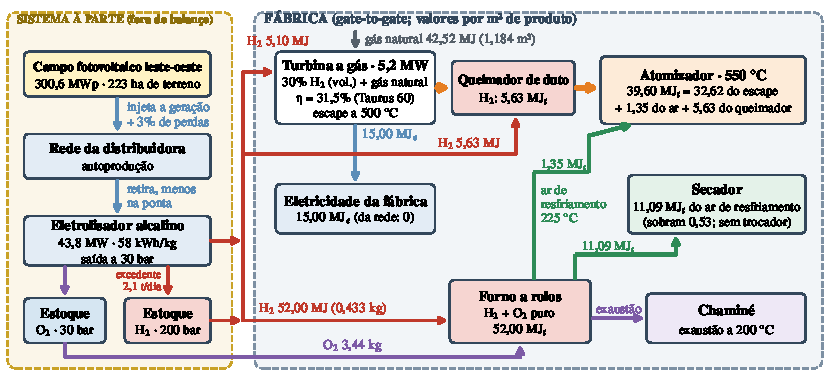
\includegraphics[width=\textwidth]{figs/fig_ciclo_rev.pdf}
\caption{Ciclo proposto: sistema à parte (campo fotovoltaico, rede, eletrolisador e estoques) e correntes da fábrica, por m² de produto. O \Ht{} vai do eletrolisador à fábrica a 30~bar; só o excedente vai ao estoque a 200~bar, que o devolve na ponta e nas paradas. Com o rendimento de catálogo da turbina, o ar de resfriamento já cobre o secador, e o trocador da exaustão é dispensado.}\label{fig:ciclo}
\end{figure*}

\subsection{Turbina a gás e atomizador}\label{sec:tg}

A turbina precisa entregar 5.208~kW no local, ou 5.600~kW nas condições ISO (Seção~\ref{sec:invest}); o menor modelo de catálogo acima disso é o Taurus 60, com 5.670~kW e consumo térmico de 11.430~kJ/kWh nas condições ISO, ou rendimento de $3.600/11.430 = 31{,}5\%$ \cite{gtw2018,solar2026}, adotado no caso-base para que o rendimento seja o da máquina orçada (35\%, valor típico de \cite{boyce2012}, fica como variante). A energia do combustível e a do escape são
\begin{align}
F_{\text{TG}} &= \frac{E_e}{\eta} = \frac{15{,}00}{0{,}315} = 47{,}62\un{MJ/m^2}, \label{eq:tg}\\
Q_{\text{esc}} &= F_{\text{TG}} - E_e = 32{,}62\un{MJ_t/m^2}, \nonumber
\end{align}
em que $E_e = 15{,}00$~\MJe/m² inclui os ventiladores. Combustores secos de baixa emissão admitem hoje de 20\% a 30\% de \Ht{} em volume \cite{netl2022}; para o combustor do Taurus 60, os 30\% precisam ser confirmados pelo fabricante. Com $x_V = 0{,}30$ e os dois PCI volumétricos na mesma base, 20~°C e 1~atm (\Ht: $10{,}78 \times 273{,}15/293{,}15 = 10{,}04$~MJ/m³, de 10,78~MJ/Nm³ \cite{cengel2013}; gás natural: 35,9~MJ/m³), a fração do \Ht{} em energia é
\begin{equation}
\begin{split}
x_E &= \frac{x_V\,\mathrm{PCI}_{\mathrm{H_2}}}{x_V\,\mathrm{PCI}_{\mathrm{H_2}} + (1-x_V)\,\mathrm{PCI}_{\text{GN}}}\\
&= \frac{0{,}30 \times 10{,}04}{0{,}30 \times 10{,}04 + 0{,}70 \times 35{,}9} = 0{,}107.
\end{split} \label{eq:xe}
\end{equation}
A turbina recebe 42,52~MJ/m² de gás natural (1,184~m³/m²) e 5,10~MJ/m² de \Ht. O escape sai a 500~°C \cite{boyce2012}, com $32{,}62 \times 1000/[1{,}10 \times 475] = 62{,}43$~kg/m² (Eq.~\eqref{eq:mq}), ou 78.036~kg/h, perto dos 78.385~kg/h a 510~°C da folha do Taurus 60 nas condições ISO \cite{solar2026}. O escape inteiro vai ao atomizador, e o restante da massa que chega a 550~°C é ar de resfriamento:
\begin{equation}
m_{\text{ar,at}} = \frac{39{,}60 \times 1000 - 62{,}43 \times 1{,}10 \times 525}{1{,}05 \times 525} = 6{,}44\un{kg/m^2}, \label{eq:marat}
\end{equation}
que leva 1,35~\MJt/m². A massa de gás, 68,9~kg/m², fica abaixo do limite da Eq.~\eqref{eq:matmax}. O queimador de duto completa a energia queimando \Ht{} no oxigênio que sobra no escape: o ar em excesso da turbina leva cerca de 10,5~kg/m² de \Ot, e o queimador consome 0,37~kg/m², menos de 4\% disso:
\begin{equation}
\begin{split}
Q_{\text{duto}} &= Q_{\text{at}} - Q_{\text{esc}} - Q_{\text{ar,at}}\\
&= 39{,}60 - 32{,}62 - 1{,}35 = 5{,}63\un{MJ_t/m^2}.
\end{split} \label{eq:duto}
\end{equation}
Restam 11,62~\MJt/m² de ar de resfriamento, mais que os 11,09 do secador: o secador não queima combustível, sobram 0,53~\MJt/m², e o trocador da exaustão é dispensado (com 35\%, o escape menor deixa ar de menos e o trocador entrega 1,48~\MJt/m²). O ar chega a 225~°C, e só a parte necessária entra no secador, diluída com ar ambiente até a temperatura de uso; essa diluição e a umidade dos gases de \Ht{} ficam para o projeto de detalhe.

\subsection{Forno com oxigênio}

Com gás natural, a exaustão do forno (153,3~kg/m²) leva o ar de combustão, $54{,}91 \times 0{,}344 \times 1{,}15 = 21{,}72$~kg/m² (0,344~kg de ar estequiométrico por MJ, estimado de \cite{cengel2013} para o metano), 1,10~kg/m² de gás natural e o ar de processo que atravessa o forno, $153{,}3 - 21{,}72 - 1{,}10 = 130{,}5$~kg/m². Com \Ot{} puro desaparece o ar de combustão, mas o ar de processo continua. Mantida a parcela que não depende da exaustão ($Q_{\text{fixo}} = 54{,}91 - 28{,}17 = 26{,}74$~\MJt/m²), a exaustão passa a ser o ar de processo a 200~°C, $a = 130{,}5 \times 1{,}05 \times 0{,}175 = 23{,}98$~\MJt/m², mais o vapor da queima do \Ht, $b = 8{,}94 \times 1{,}90 \times 0{,}175/120 = 0{,}0248$~\MJt{} por MJ de \Ht, de modo que
\begin{equation}
Q_F = \frac{Q_{\text{fixo}} + a}{1 - b} = \frac{26{,}74 + 23{,}98}{1 - 0{,}0248} \approx 52{,}00\un{MJ_t/m^2}, \label{eq:forno}
\end{equation}
2,91~\MJt/m² (5\%) a menos que com gás natural. A Fig.~\ref{fig:calor} resume as fontes de calor das três operações nos três casos.

\begin{figure}[!t]
\centering
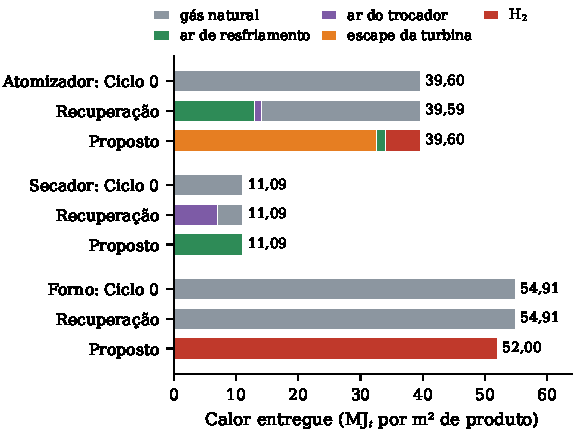
\includegraphics[width=\columnwidth]{figs/fig_calor_rev.pdf}
\caption{Fontes de calor do atomizador, do secador e do forno no ciclo 0, com recuperação de calor e no ciclo proposto.}\label{fig:calor}
\end{figure}

\subsection{Hidrogênio, eletrolisador e campo fotovoltaico}

O consumo de \Ht{} soma a turbina, o queimador de duto e o forno:
\begin{equation}
m_{\mathrm{H_2}} = \frac{5{,}10 + 5{,}63 + 52{,}00}{120} = 0{,}523\un{kg/m^2}, \label{eq:mh2}
\end{equation}
ou 15,7~t/dia. A eletrólise produz 7,94~kg de \Ot{} por kg de \Ht: 4,15~kg/m², dos quais o forno usa 3,44 e sobram 0,71 para venda. O estoque guarda um dia de consumo a 200~bar (hipótese conservadora: cobre a ponta e as paradas), 1.089~m³.

Adotou-se eletrolisador alcalino, mais de 90\% da fabricação chinesa \cite{iea2025a}, com 58~kWh/kg: a IEA dá eficiência de 58\% (PCI) para a China em 2024, ou $120/(0{,}58 \times 3{,}6) = 57{,}5$~kWh/kg \cite{iea2025b}, e só o excedente que vai ao estoque, $15{,}7 \times (1 - 21{,}86 \times 0{,}95/24) = 2{,}1$~t/dia, é comprimido de 30 a 200~bar, com 0,995~kWh/kg (dois estágios e 75\% de rendimento, hipótese), ou 0,13~kWh/kg na média; o total, arredondado para cima, dá os 58~kWh/kg. A eletricidade necessária é de $0{,}523 \times 58 = 30{,}32$~kWh/m², ou 909,6~MWh/dia.

Um eletrolisador ligado direto ao campo, sem baterias, teria de acompanhar o pico de geração, cerca de 0,72 vez a potência do campo na série horária do PVGIS \cite{pvgis2026}, e teria fator de capacidade de só 18\% ($1.137{,}5/(0{,}72 \times 8.760)$). Por isso o campo e o eletrolisador são ligados à rede da distribuidora como autoprodução: o campo injeta a sobra do meio-dia e do verão, e o eletrolisador retira a mesma energia ao longo do dia e do ano, desligado só na ponta dos dias úteis, das 18h30 às 21h30 \cite{aneel2026,aneel2021}. Com $h_{\text{op}} = 24 - 3\times 5/7 = 21{,}86$~h/dia e disponibilidade de 95\% (hipótese),
\begin{equation}
P_{\text{ELZ}} = \frac{909{,}6}{21{,}86 \times 0{,}95} = 43{,}8\un{MW}. \label{eq:pelz}
\end{equation}
Para o campo, adotou-se 1.300~kWh/\allowbreak{}(kWp·ano) com placas ao norte, dentro da faixa de Santa Catarina, de 1.222 a 1.423 \cite{canalsolar2022}, e 12,5\% a menos no leiaute leste-oeste \cite{pvmag2021}, que sobe a densidade de cerca de 0,87~MWp/ha \cite{bolinger2022} para 1,35~MWp/ha \cite{pvmag2021}. Com 3\% de perdas na rede (hipótese),
\begin{equation}
P_{\text{FV}} = \frac{909{,}6 \times 365 \times 1{,}03}{1.137{,}5} = 300{,}6\un{MWp}, \label{eq:pfv}
\end{equation}
ou 484,9 mil placas de 620~Wp em 223~ha.

\subsection{Fechamento e resultados}

A energia que entra na planta iguala a demanda térmica mais a eletricidade gerada,
\begin{equation}
m_{\mathrm{H_2}}\,\mathrm{PCI}_{\mathrm{H_2}} + F_{\text{GN}} + Q_{\text{rec}} = Q_F + Q_{\text{at}} + Q_{\text{sec}} + E_e, \label{eq:fecha}
\end{equation}
com 62,73~MJ/m² de \Ht, 42,52 de gás natural e 12,44 de calor recuperado ($1{,}35 + 11{,}09$) de um lado, e 52,00, 39,60, 11,09 e 15,00 do outro: 117,7~MJ/m² nos dois. O único combustível fóssil é o gás natural da turbina:
\begin{equation}
\mathrm{CO_2}_{,P} = 42{,}52 \times 0{,}0561 = 2{,}39\un{kg/m^2}, \label{eq:co2p}
\end{equation}
61\% a menos que o ciclo 0 (Fig.~\ref{fig:co2} e Tabela~\ref{tab:comparacao}). A energia que entra na fábrica cai 12\%, mas, contando a eletricidade da fotovoltaica no lugar do \Ht, o sistema consome 151,7~MJ/m², 26\% a mais que o ciclo 0 (155,0 e +29\% com as perdas na rede). Com a mediana de 48~g~\COt{}e/kWh do ciclo de vida da fotovoltaica \cite{schlomer2014}, o \Ht{} tem $58 \times 1{,}03 \times 0{,}048 = 2{,}87$~kg~\COt{}e/kg, abaixo dos 7~kg que definem o hidrogênio de baixa emissão na Lei nº 14.948/2024 \cite{lei14948}, por balanço anual.

\begin{figure}[!t]
\centering
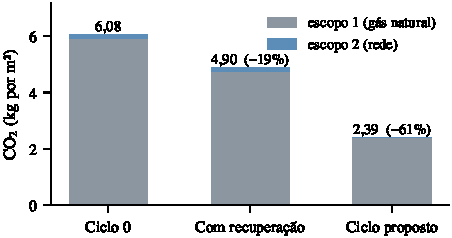
\includegraphics[width=\columnwidth]{figs/fig_co2_rev.pdf}
\caption{Emissões de \COt{} por m² de produto.}\label{fig:co2}
\end{figure}

\begin{table}[!t]
\centering
\caption{Indicadores por m² de produto}\label{tab:comparacao}
\footnotesize
\begin{tabular}{L{3.85cm}rrr}
\toprule
\textbf{Indicador} & \textbf{Ciclo 0} & \textbf{Proposto} & \textbf{Variação}\\ \midrule
\COt{} da energia, escopos 1 e 2 (kg) & 6,08 & 2,39 & −61\%\\
Gás natural (m³) & 2,941 & 1,184 & −60\%\\
Eletricidade da rede (kWh) & 4,00 & 0\textsuperscript{a} & −100\%\\
Energia que entra na fábrica (MJ) & 119,99 & 105,25 & −12\%\\
Energia com a FV, sem / com perdas (MJ) & 119,99 & 151,7 / 155,0 & +26 / +29\%\\
Calor do forno descartado (\MJt) & 43,43 & 28,08 & −35\%\\
Eficiência exergética (Seção~\ref{sec:exergia}) & 31,0\% & 24,6\% & −6,4 p.p.\\
\Ht{} (kg) & -- & 0,523 & novo\\
Eletricidade da FV à parte (kWh) & -- & 30,32 & novo\\
\Ot{} disponível para venda (kg) & -- & 0,71 & novo\\
\bottomrule
\multicolumn{4}{L{7.6cm}}{\scriptsize \textsuperscript{a} Em regime; nas horas acima de cerca de 26,6~°C a turbina não cobre toda a demanda (Seção~\ref{sec:invest}).}\\
\end{tabular}
\end{table}

\section{Avaliação econômica}

\subsection{Custo de investimento}\label{sec:invest}

Sem preço comercial para boa parte dos equipamentos, o custo de cada item foi estimado por correlações e referências da literatura, em quatro parcelas. (1) O equipamento na origem é levado a dólares de 2026 pelo índice CEPCI,
\begin{equation}
C_{2026} = C_{\text{base}}\, c\, \frac{\mathrm{CEPCI}_{2026}}{\mathrm{CEPCI}_{\text{base}}}, \label{eq:cepci}
\end{equation}
em que $c$ é o câmbio para dólar dos itens cotados em libras. Os índices são 397 em 2001 \cite{turton2018}, 525,4 em 2007 \cite{chemeng2026}, 603,1 em 2018 \cite{venturini2021}, 816,0 em 2022 e 798,8 em 2024 \cite{toweringskills}, e 500 nas correlações de \cite{seider2017}; para 2026, 811,6, o de 2024 com a alta de 1,6\% de 2025 \cite{cepci2026} (hipótese). (2) Sobre o equipamento importado soma-se 80\%, orientação da disciplina com origem no fator de 0,87 de \cite{izidoro2016}; o fabricado no Brasil leva o fator de localização de 1,14 \cite{towler2022}. (3) A instalação e (4) os indiretos também são multiplicados por 1,14. A fotovoltaica é a exceção: o preço da EPE já é do Brasil, convertido a 6,10~R\$/US\$ e atualizado só pelo CEPCI. A operação e manutenção e os encargos da fotovoltaica, também da EPE, usam o mesmo câmbio; os demais custos anuais e os totais em reais usam 5,3488~R\$/US\$ \cite{agrolink2026}.

A potência de catálogo é dada a 15~°C; com perda de 0,7\% por °C acima disso (hipótese, dentro dos 5\% a 10\% a cada 10~°C de \cite{wartsila}) e 25~°C no mês mais quente (Florianópolis: 24,7~°C em fevereiro \cite{embrapa}),
\begin{equation}
P_{\text{ISO}} = \frac{P_{\text{TG}}}{1 - k\,(T_{\text{loc}} - 15)} = \frac{5.208}{1 - 0{,}007 \times 10} = 5.600\un{kW}. \label{eq:piso}
\end{equation}
O Taurus 60 (5.670~kW ISO) não chega aos 5.208~kW nas horas acima de cerca de 26,6~°C (a 30~°C, entrega 2,6\% a menos); nessas horas a diferença viria da rede. A Tabela~\ref{tab:bases} mostra a base de cada item e a Fig.~\ref{fig:invest}, a composição.

\begin{table*}[!t]
\centering
\caption{Base de custo e investimento de cada item (US\$ milhões de 2026)}\label{tab:bases}
\footnotesize
\begin{tabular}{L{4.1cm}L{10.0cm}L{1.5cm}r}
\toprule
\textbf{Item} & \textbf{Base de custo (valor e ano da base)} & \textbf{Origem} & \textbf{Total}\\ \midrule
Campo fotovoltaico (300,6~MWp) & R\$~3.000/kW de dez./2024, a referência mais baixa da EPE \cite{epe2025}; ÷ 6,10~R\$/US\$ e CEPCI: 499,7~US\$/kW em 2026; divisão em módulos e inversores, BoS, instalação e indiretos da IRENA \cite{irena2025} & preço local & 150,2\\
Eletrolisador alcalino (43,8~MW) & 900~US\$/kW instalado na China em 2024 \cite{iea2025a}, US\$~39,4 milhões; 40\% equipamento e 60\% de engenharia, obra e contingência \cite{iea2025a}, repartidos em 22,5\% de instalação e 37,5\% de indiretos, na proporção de \cite{james2024} & importado & 56,2\\
Estoque de \Ht{} (15,7~t a 200~bar, 1 dia) & 635~US\$/kg armazenado em vasos de aço (2007), US\$~10,0 milhões; instalação de 30\% \cite{nrel2014} & importado & 33,0\\
Turbina a gás (5.670~kW ISO) & Taurus 60: US\$~4,32 milhões (2018), só o equipamento; demais custos iguais ao equipamento \cite{gtw2018} & importado & 17,1\\
Forno: queimadores de \Ht{} + \Ot{} (18,1~MWt) & conversão para \Ht{} por porte, em £ de 2022 \cite{arup2022}, a 1,2366 US\$/£ \cite{valutafx}, com fator 2 para a oxicombustão (hipótese): £~1,01 milhão; instalação de 30\% \cite{nrel2014} & importado & 2,66\\
Queimador de duto a \Ht{} (2,0~MWt) & idem, sem o fator 2: £~29,5 mil & importado & 0,08\\
Compressor de \Ht{} (101~kW, 30 para 200~bar, só o excedente) & US\$~146,6 mil (CEPCI 500) \cite{seider2017}; instalação de 30\% \cite{nrel2014} & importado & 0,51\\
Ventilador da recuperação (64.126 cfm) & US\$~18,1 mil (CEPCI 500) \cite{seider2017}; instalação de 30\% \cite{nrel2014} & nacional & 0,04\\
Dutos, tubulações de \Ht{} e \Ot{} e instrumentação & 15\% do custo instalado da turbina, do forno, do queimador de duto e do ventilador (hipótese); trocador dispensado (Seção~\ref{sec:tg}) & -- & 2,98\\
\midrule
\textbf{Total} (fábrica 22,9; sistema à parte 239,9) & & & \textbf{262,8}\\
\bottomrule
\end{tabular}
\end{table*}

\begin{figure}[!t]
\centering
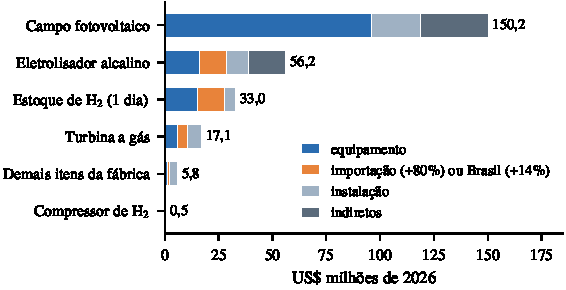
\includegraphics[width=\columnwidth]{figs/fig_invest_rev.pdf}
\caption{Investimento por item e por parcela. Nos itens nacionais, a segunda parcela é o fator de localização (+14\%). Os demais itens da fábrica reúnem forno, queimador de duto, ventilador e dutos; os dutos aparecem como instalação.}\label{fig:invest}
\end{figure}

O investimento total é de US\$~262,8 milhões (R\$~1,41 bilhão), 91\% no sistema à parte: o campo fotovoltaico é o maior item (57\%), seguido do eletrolisador (21\%) e do estoque de \Ht{} (13\%). Com o fator Brasil e a importação, o eletrolisador sai a 1.284~US\$/kW em Tijucas, abaixo dos 1.500 a 2.400~US\$/kW que a IEA estima para eletrolisadores chineses instalados fora da China \cite{iea2025a}; o resultado é otimista nesse item.

\subsection{Fluxo de caixa e critérios}\label{sec:fluxo}

A análise segue Lora e Nascimento \cite{lora2004}, em termos reais, antes de impostos, com taxa de 8\% ao ano e vida de 25 anos \cite{epe2025}. O benefício anual é o que a fábrica deixa de comprar em relação ao ciclo 0: 19,2 milhões de m³ de gás natural, US\$~12,5 milhões, a R\$~3,4865/m³ em média na tarifa industrial TG1 da SCGÁS, cobrada em cascata por faixa de consumo diário \cite{scgas2026} (o ciclo 0 usa 88,2~mil~m³/dia, uma fatura de R\$~313,6~mil por dia, e o proposto, 35,5~mil, R\$~129,8~mil por dia; o gás evitado sai das faixas de 25.001 a 50.000~m³/dia, a R\$~3,5563/m³, e de 50.001 a 100.000, a R\$~3,4601/m³), e 43,8~GWh a R\$~600/MWh (hipótese), US\$~4,9 milhões. Os custos anuais são a operação e manutenção da fotovoltaica, R\$~60/(kW·ano) \cite{epe2025} (US\$~3,0 milhões); a manutenção dos demais itens, 1,5\% ao ano do investimento sem a fotovoltaica \cite{lora2004} (US\$~1,7 milhão); o uso da rede, US\$~6,6 milhões (demanda do eletrolisador, parcela de energia e tarifa da usina \cite{aneel2026}, e acerto na CCEE com o preço horário de 2024 e 2025 \cite{ccee2025} sobre os 60,6\% da energia que passam pela rede no perfil do campo \cite{pvgis2026}); a troca das pilhas, que a 7.580~h/ano ocorre nos anos 7, 14 e 20, cada uma a 17,5\% do custo do eletrolisador, US\$~11,2 milhões em valor presente, ou US\$~1,0 milhão por ano; e os encargos da fotovoltaica, R\$~120/(kW·ano) \cite{epe2025} a 6,10~R\$/US\$, menos os R\$~48/(kW·ano) da tarifa da usina, já contados no uso da rede a 5,3488, US\$~3,2 milhões. O fluxo anual é
\begin{equation}
\begin{split}
\mathrm{FC} &= 12{,}5 + 4{,}9 - 3{,}0 - 1{,}7 - 6{,}6 - 1{,}0 - 3{,}2\\
&= 1{,}91\un{US\$\ milhão/ano}
\end{split} \label{eq:fc}
\end{equation}
(termos arredondados; a soma é feita sem arredondar). Com o fator de recuperação de capital
\begin{equation}
\mathrm{FRC} = \frac{i\,(1+i)^n}{(1+i)^n - 1} = 0{,}0937, \label{eq:frc}
\end{equation}
o valor presente líquido, em US\$ milhões, é
\begin{equation}
\mathrm{VPL} = -I + \frac{\mathrm{FC}}{\mathrm{FRC}} = -262{,}8 + \frac{1{,}91}{0{,}0937} = -242{,}4. \label{eq:vpl}
\end{equation}
O custo nivelado do \Ht{} considera só o sistema à parte ($I_s$ = US\$~239,9 milhões), com a sua manutenção, o uso da rede, as pilhas e os encargos, e a produção anual de 5,72 milhões de kg:
\begin{equation}
\begin{split}
\mathrm{LCOH} &= \frac{I_s\,\mathrm{FRC} + \mathrm{O\&M}_s}{m_{\mathrm{H_2},\text{ano}}}\\
&= \frac{22{,}5 + 15{,}2}{5{,}72} = 6{,}58\un{US\$/kg}.
\end{split} \label{eq:lcoh}
\end{equation}
O custo de evitar \COt{} é o valor anual uniforme com o sinal trocado, $-\mathrm{VPL} \times \mathrm{FRC} = 22{,}7$ milhões de US\$/ano, dividido pelo \COt{} evitado, $(6{,}08 - 2{,}39) \times 10{,}95$ milhões de m² = 40,4~mil~t/ano: 562~US\$/t.

\begin{table}[!t]
\centering
\caption{Indicadores econômicos (antes de impostos)}\label{tab:econ}
\footnotesize
\begin{tabular}{L{5.2cm}r}
\toprule
\textbf{Indicador} & \textbf{Valor}\\ \midrule
Investimento (US\$ milhões) & 262,8\\
Fluxo de caixa anual (US\$ milhões) & 1,9\\
Valor presente líquido (US\$ milhões) & −242,4\\
Taxa interna de retorno (\% ao ano) & −10,3\\
Custo nivelado do \Ht{} (US\$/kg) & 6,58\\
Custo de evitar \COt{} (US\$/t) & 562\\
Custo a mais por m² de produto (R\$) & 11,09\\
Preço do gás que zera o VPL (R\$/m³) & 9,80\\
VPL depois de impostos (US\$ milhões) & −211,2\\
TIR depois de impostos (\% ao ano) & −5,3\\
\bottomrule
\end{tabular}
\end{table}

O projeto não se paga (Tabela~\ref{tab:econ}): o benefício anual mal cobre os custos anuais, e o investimento não volta (Fig.~\ref{fig:fluxo}). Fora dos anos de troca das pilhas, o fluxo é de US\$~3,0 milhões por ano; com as três trocas, de US\$~9,8 milhões cada, o acumulado sem desconto termina em −US\$~218,3 milhões (volta só 17\% do investimento) e a 8\% ao ano, no VPL; a TIR é de −10,3\% ao ano. Depois de impostos, com depreciação linear de 4\% ao ano \cite{lora2004} e IR e CSLL de 34\% \cite{epe2025}, o VPL melhora para −US\$~211,2 milhões, porque o prejuízo fiscal é abatido do lucro da fábrica (hipótese). Ficam fora da conta, e a tornariam pior, os estoques de \Ot, a subestação e a linha de conexão, a água, o pessoal e o financiamento.

\begin{figure}[!t]
\centering
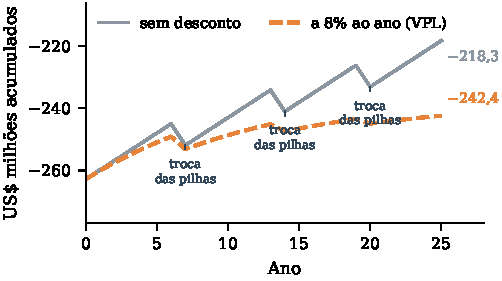
\includegraphics[width=\columnwidth]{figs/fig_fluxo_rev.pdf}
\caption{Dinheiro acumulado do projeto em 25 anos, sem desconto e a 8\% ao ano (VPL), com as trocas das pilhas nos anos em que ocorrem.}\label{fig:fluxo}
\end{figure}

\subsection{Cenários e sensibilidade}

O preço do gás natural forma 72\% do benefício anual. Sem crédito de carbono, o VPL se anula com o gás a R\$~9,80/m³, 2,8 vezes o preço médio evitado de hoje; com o gás pelo dobro, o VPL é de −US\$~108,5 milhões, e pelo triplo, de +US\$~25,3 milhões, com TIR de 9,1\%, pouco acima da taxa (Tabela~\ref{tab:cenarios}). A tarifa também conta: na de matéria-prima (TMP) \cite{scgas2026b}, usada nas versões anteriores, o VPL seria de −US\$~254,7 milhões; se o gás da turbina fosse enquadrado na tarifa de geração distribuída (TGG) \cite{scgas2026c}, faturada pela faixa do consumo total (leitura e enquadramento são hipóteses), seria de −US\$~227,8 milhões. Baratear o investimento sozinho não basta: sem o acréscimo de importação, o VPL é de −US\$~202,9 milhões; com o gás pelo triplo e o investimento pela metade, chega a +US\$~171,3 milhões. Para 2030, com o eletrolisador chinês a 675~US\$/kW e a fotovoltaica com o fator $18/26 = 0{,}69$, a queda que a IEA projeta para o custo da energia solar na América Latina \cite{iea2025b} (hipótese), o investimento cai para US\$~202,5 milhões e o \Ht{} para 5,51~US\$/kg, mas o VPL ainda é de −US\$~177,1 milhões. Variado sozinho na sua faixa (Fig.~\ref{fig:tornado}), nenhum parâmetro deixa o VPL positivo; o preço da fotovoltaica pesa mais (−US\$~227 a −368 milhões), seguido do preço do eletrolisador e do acréscimo de importação. Como o fluxo anual é quase nulo, a taxa e a vida útil quase não mudam o VPL: o resultado é dado pelo investimento.

\begin{table}[!t]
\centering
\caption{Cenários, antes de impostos: VPL em US\$ milhões, TIR em \% ao ano e \Ht{} em US\$/kg}\label{tab:cenarios}
\footnotesize
\begin{tabular}{L{4.6cm}rrr}
\toprule
\textbf{Cenário} & \textbf{VPL} & \textbf{TIR} & \textbf{\Ht}\\ \midrule
Caso-base & −242,4 & −10,3 & 6,58\\
Gás natural pelo dobro & −108,5 & 2,6 & 6,58\\
Gás natural pelo triplo & +25,3 & 9,1 & 6,58\\
Sem acréscimo de importação & −202,9 & −8,0 & 6,06\\
Eletrolisador a 600~US\$/kW & −216,9 & −8,5 & 6,16\\
Eletrolisador a 1.200~US\$/kW & −267,9 & −12,6 & 7,00\\
Eletrolisador a 2.300~US\$/kW (fora da China) & −361,3 & -- & 8,53\\
Tarifa de matéria-prima (TMP) & −254,7 & −14,6 & 6,58\\
Gás da turbina na tarifa TGG & −227,8 & −7,5 & 6,58\\
Investimento pela metade e gás pelo triplo & +171,3 & 21,4 & 4,41\\
2030 (eletrolisador e FV mais baratos) & −177,1 & −7,8 & 5,51\\
\bottomrule
\multicolumn{4}{L{7.6cm}}{\scriptsize --: TIR inexistente (fluxo anual negativo).}\\
\end{tabular}
\end{table}

\begin{figure}[!t]
\centering
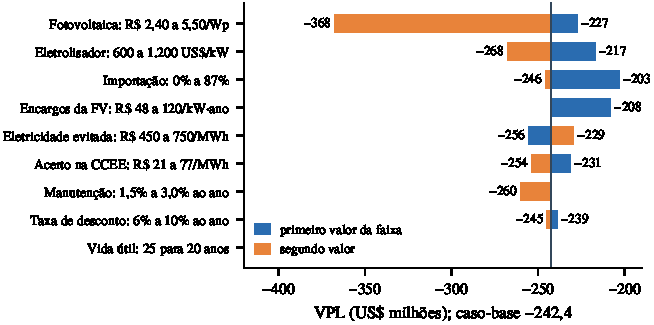
\includegraphics[width=\columnwidth]{figs/fig_tornado_rev.pdf}
\caption{Sensibilidade do VPL a cada parâmetro, com os demais no valor adotado.}\label{fig:tornado}
\end{figure}

As hipóteses técnicas, também uma por vez, mudam pouco a conclusão (Tabela~\ref{tab:robustez}). Com o rendimento de 35\%, o \COt{} cai para 2,15~kg/m², mas o VPL piora US\$~6 milhões, porque o escape menor pede mais \Ht{} no queimador de duto. A eletrólise de 2030 na China, 62\% (PCI) \cite{iea2025b}, ou 54~kWh/kg com a compressão, melhora o VPL em US\$~25 milhões; as frações de calor nas pontas das faixas mudam o \Ht{} em 3\%. Guardar no estoque só o excedente, sem reserva para paradas longas, melhora o VPL em US\$~33 milhões.

\begin{table}[!t]
\centering
\caption{Robustez: \Ht{} e \COt{} fóssil em kg/m², VPL em US\$ milhões e custo do \Ht{} em US\$/kg}\label{tab:robustez}
\footnotesize
\begin{tabular}{L{3.3cm}rrrr}
\toprule
\textbf{Variante} & \textbf{\Ht} & \textbf{\COt} & \textbf{VPL} & \textbf{US\$/kg}\\ \midrule
Caso-base (31,5\%) & 0,523 & 2,39 & −242,4 & 6,58\\
Turbina a 35\% \cite{boyce2012} & 0,542 & 2,15 & −248,0 & 6,58\\
Eletrólise de 2030 (54~kWh/kg) & 0,523 & 2,39 & −217,3 & 6,17\\
Frações de calor 49/39/12\% & 0,506 & 2,39 & −229,6 & 6,58\\
Frações de calor 55/36/9\% & 0,540 & 2,39 & −255,5 & 6,58\\
Estoque só do excedente & 0,523 & 2,39 & −209,3 & 6,04\\
Pilha a 15\% / 20\% & 0,523 & 2,39 & −240,8 / −244,0 & 6,56 / 6,61\\
\bottomrule
\end{tabular}
\end{table}

\subsection{Incerteza conjunta}\label{sec:mc}

Para medir o efeito das incertezas juntas, sortearam-se 10.000 combinações de dez grupos de hipóteses, cada um numa faixa com fonte ou declarada como hipótese (Tabela~\ref{tab:mc_ent}), e para cada combinação refez-se todo o cálculo: o ciclo proposto, o tamanho do campo e do eletrolisador, o investimento e o fluxo de caixa, com as pilhas e os encargos. Usou-se distribuição triangular, com a moda no caso-base, quando ele está dentro da faixa, e uniforme quando ele está numa ponta ou quando a faixa só tem dois valores observados; as frações de calor foram sorteadas por igual na região em que as três faixas valem e somam 100\%. As hipóteses foram tomadas como independentes. Taxa, vida útil, câmbio e preço da eletricidade ficam fixos. O preço do gás natural não foi sorteado, por falta de fonte para a sua distribuição futura: como o VPL é linear nele, cada combinação dá o preço que zera o VPL, e a distribuição desse preço dá a probabilidade de o projeto se pagar para qualquer preço do gás (Fig.~\ref{fig:mc}b). O gerador é o mulberry32, com semente 20261126; com a semente 20261127, nenhum percentil da Tabela~\ref{tab:mc_sai} muda mais de 0,51\%.

\begin{table}[!b]
\centering
\caption{Hipóteses sorteadas no Monte Carlo (triangular: mínimo / moda / máximo, com a moda no caso-base)}\label{tab:mc_ent}
\footnotesize
\begin{tabular}{L{2.2cm}L{2.55cm}L{3.05cm}}
\toprule
\textbf{Hipótese} & \textbf{Distribuição e faixa} & \textbf{Origem}\\ \midrule
Rendimento elétrico da turbina & uniforme, 31,5 a 35\% & catálogo \cite{gtw2018}; \cite{boyce2012}\\
Queima / atomização / secagem & uniforme, 49--55 / 36--39 / 9--12\%, soma 100\% & faixas realistas em \cite{rigobelo2026}\\
Consumo do eletrolisador & uniforme, 54 a 58~kWh/kg & eficiência de 2030 e de 2024 na China \cite{iea2025b}, mais a compressão\\
Eletrolisador instalado na China & triangular, 600 / 900 / 1.200~US\$/kW & \cite{iea2025b,iea2025a}\\
Campo fotovoltaico & triangular, 2,40 / 3,00 / 5,50~R\$/Wp & 2,40: \cite{greener2026}; 3,00 e 5,50: \cite{epe2025}\\
Acréscimo de importação & triangular, 0 / 80 / 87\% & 0: hipótese; 80\%: disciplina; 87\%: \cite{izidoro2016}\\
Manutenção dos demais itens & uniforme, 1,5 a 3,0\% ao ano & \cite{lora2004}; 3,0\%: o da eletrólise \cite{iea2025b} (hipótese)\\
Acerto na CCEE, por MWh que passa pela rede & uniforme, 20,5 a 77,1~R\$/MWh & preços horários de 2024 e de 2025 \cite{ccee2025}\\
Custo da pilha & uniforme, 15 a 20\% do eletrolisador & \cite{iea2025a}\\
Encargos da fotovoltaica & uniforme, 48 a 120~R\$/(kW·ano) & 48: só a tarifa da usina \cite{aneel2026}; 120: \cite{epe2025}\\
\bottomrule
\end{tabular}
\end{table}

\begin{figure*}[!t]
\centering
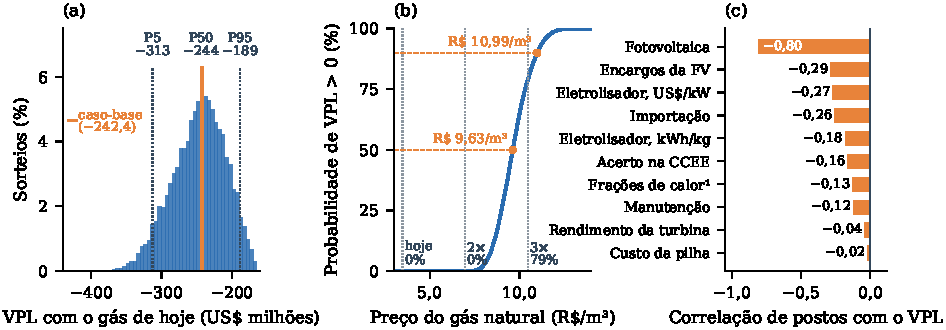
\includegraphics[width=\textwidth]{figs/fig_mc_rev.pdf}
\caption{Monte Carlo com 10.000 combinações das hipóteses da Tabela~\ref{tab:mc_ent}: (a) distribuição do VPL com o gás natural ao preço de hoje; (b) probabilidade de o VPL ser positivo em função do preço do gás; (c) correlação de postos de cada hipótese com o VPL (¹ frações de calor representadas pela da queima).}\label{fig:mc}
\end{figure*}

\begin{table}[!t]
\centering
\caption{Monte Carlo: caso-base e percentis 5, 50 e 95}\label{tab:mc_sai}
\footnotesize
\begin{tabular}{L{3.55cm}rrrr}
\toprule
\textbf{Indicador} & \textbf{Base} & \textbf{P5} & \textbf{P50} & \textbf{P95}\\ \midrule
\Ht{} (kg/m²) & 0,523 & 0,517 & 0,532 & 0,548\\
\COt{} fóssil (kg/m²) & 2,39 & 2,16 & 2,26 & 2,37\\
\COt{} (mil~t/ano) & 26,1 & 23,6 & 24,8 & 26,0\\
Investimento (US\$ milhões) & 262,8 & 239,2 & 282,3 & 346,7\\
VPL (US\$ milhões) & −242,4 & −312,6 & −243,9 & −188,6\\
Custo do \Ht{} (US\$/kg) & 6,58 & 5,72 & 6,56 & 7,65\\
Custo de evitar \COt{} (US\$/t) & 562 & 422 & 547 & 701\\
Gás que zera o VPL (R\$/m³) & 9,80 & 8,22 & 9,63 & 11,36\\
\bottomrule
\end{tabular}
\end{table}

Com o gás de hoje, nenhuma das 10.000 combinações tem VPL positivo (Tabela~\ref{tab:mc_sai} e Fig.~\ref{fig:mc}a): em 90\% delas o VPL fica entre −US\$~313 milhões e −US\$~189 milhões, e em 0,1\% a TIR nem existe. Com as pilhas e os encargos no caso-base, ele fica no meio da distribuição (51\% das combinações abaixo dele). A fotovoltaica explica a maior parte da dispersão (correlação de postos de −0,80 com o VPL), seguida dos encargos da fotovoltaica, do preço do eletrolisador e da importação; o rendimento da turbina, as frações de calor e o custo da pilha pesam pouco. Para o projeto se pagar com 50\% de probabilidade, o gás teria de custar R\$~9,63/m³, 2,8 vezes o de hoje; com 90\%, R\$~10,99/m³, 3,2 vezes. Com o gás pelo dobro, nenhuma combinação se paga; pelo triplo, 79\%. Nas emissões, o que conta é o rendimento da turbina: abaixo de 32,9\%, o que ocorre em 41\% das combinações e no caso-base, o ciclo proposto passa de 25~mil~t/ano e teria de conciliar as emissões no SBCE \cite{lei15042}. As probabilidades valem para as distribuições e a independência adotadas: mostram que a conclusão não depende de uma combinação particular de hipóteses, e não são uma previsão de mercado.

\subsection{Otimização}\label{sec:otim}

Duas escolhas foram otimizadas com o mesmo modelo: o tamanho do eletrolisador, com as horas em que ele opera, e o uso do \Ht{} na fábrica. O campo é dado pela energia do ano (Eq.~\eqref{eq:pfv}) e o estoque guarda um dia por confiabilidade, e não por custo.

\textit{Tamanho do eletrolisador.} O do caso-base é o menor possível: opera todas as horas fora da ponta. Um eletrolisador maior pode operar só nas horas de PLD mais baixo; o tamanho foi variado de 1 a 2 vezes o mínimo, com o despacho de menor custo em cada mês pelos preços médios de 2024 e 2025 \cite{ccee2025}. Com o dobro do tamanho, o acerto cai de 29,6 para 7,0~R\$ por MWh consumido, mas o uso da rede quase não muda (de US\$~6,64 milhões para 6,48 a 6,61 milhões por ano), porque a demanda contratada cresce com o tamanho, e o investimento sobe US\$~5,9 milhões a cada 10\%. O VPL piora US\$~5,3 milhões nos primeiros 10\% e chega a −US\$~305,5 milhões com o dobro (Fig.~\ref{fig:otim}a); o mínimo continua ótimo com os preços de 2025 e com o eletrolisador a 600~US\$/kW.

\begin{figure*}[!t]
\centering
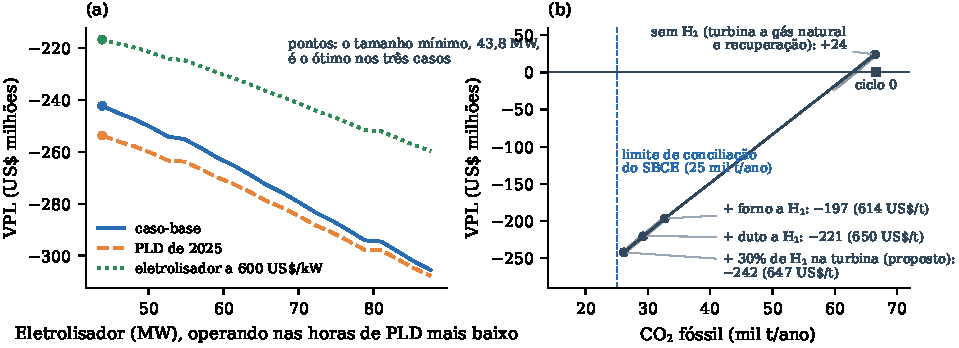
\includegraphics[width=\textwidth]{figs/fig_otim_rev.pdf}
\caption{Otimização: (a) VPL em função do tamanho do eletrolisador, que opera em cada mês nas horas de PLD mais baixo; (b) VPL e \COt{} fóssil das 286 configurações de uso do \Ht{} (círculos cinzentos, quase todos sobre a reta) e caminho do sem \Ht{} ao ciclo proposto, com o custo de cada passo por tonelada de \COt{} evitada.}\label{fig:otim}
\end{figure*}

\textit{Uso do \Ht.} Foram combinados o forno (\Ht{} com \Ot{} ou gás natural com ar), a fração do queimador de duto suprida por \Ht{} (0 a 100\%) e o \Ht{} na turbina (0 a 30\% em volume), em 286 configurações; com o forno a gás, não há conversão de queimadores, e o duto só a gás usa o queimador do atomizador (hipóteses). Sem nenhum \Ht, com a turbina a gás natural e a recuperação, o VPL é de +US\$~24,2 milhões (zera com a eletricidade a R\$~323/MWh), mas o \COt{} quase não cai (6,07~kg/m²): a turbina troca por gás a eletricidade da rede, de fator de emissão baixo \cite{mcti2024}, e o seu escape ocupa o lugar do ar recuperado no atomizador. A partir daí, cada uso do \Ht{} custa quase o mesmo por tonelada de \COt{} evitada (Tabela~\ref{tab:otim}): 614~US\$/t no forno, 650 no duto e 647 na turbina (sem converter o forno, o duto e a turbina custariam 670 e 669~US\$/t), sobre uma mesma reta, a no máximo US\$~3 milhões dela (Fig.~\ref{fig:otim}b), com 619~US\$/t do sem \Ht{} ao proposto: não há ótimo intermediário. Até 5,47~kg/m² o maior VPL vem do duto e da turbina, com o forno a gás; abaixo disso entra o forno, de uma vez (tudo ou nada, hipótese). Nenhuma configuração fica abaixo do limite do SBCE: o menor valor, o do proposto, é de 26,1~mil~t/ano, e chegar a 25~mil exigiria 38\% de \Ht{} na turbina, acima do que os combustores admitem hoje \cite{netl2022}.

\begin{table}[!t]
\centering
\caption{Uso do \Ht, do sem \Ht{} ao proposto: \Ht{} e \COt{} fóssil em kg/m², VPL em US\$ milhões e custo do passo em US\$/t de \COt{} evitada}\label{tab:otim}
\footnotesize
\begin{tabular}{L{3.4cm}rrrr}
\toprule
\textbf{Configuração} & \textbf{\Ht} & \textbf{\COt} & \textbf{VPL} & \textbf{US\$/t}\\ \midrule
Sem \Ht{} (turbina a gás natural e recuperação) & 0 & 6,07 & +24,2 & --\\
+ forno a \Ht{} com \Ot & 0,433 & 2,99 & −196,8 & 614\\
+ queimador de duto a \Ht & 0,480 & 2,67 & −220,8 & 650\\
+ 30\% de \Ht{} na turbina (proposto) & 0,523 & 2,39 & −242,4 & 647\\
\bottomrule
\end{tabular}
\end{table}

\section{Análise exergética}\label{sec:exergia}

\textit{Método.} A exergia de cada corrente foi calculada com o estado morto a 25~°C e 1~atm. Para os combustíveis, usou-se a exergia química padrão \cite{bejan1996}: 831,65~kJ/mol para o metano, tomada para o gás natural (1,037 vezes o PCI, hipótese), 236,09~kJ/mol para o \Ht{} (117,1~MJ/kg, 0,976 vezes o PCI) e 3,97~kJ/mol para o \Ot. A eletricidade é exergia pura. A exergia de um gás aquecido, com $c_p$ constante, é a fração $1 - T_0\ln(T/T_0)/(T-T_0)$ do seu calor sensível: 0,138 a 125~°C, 0,165 a 150~°C, 0,235 a 225~°C, 0,402 a 500~°C e 0,423 a 550~°C. Os produtos são os mesmos nos três cenários: a eletricidade de processo (14,40~\MJe/m²), o gás quente na entrada do atomizador (39,60~\MJt{} a 550~°C) e do secador (11,09~\MJt{} a 125~°C, a consigna dos gases na saída de um secador vertical de porcelanato \cite{mezquita2012}, tomada como o nível de temperatura do calor útil, hipótese conservadora), e a exergia retida nas transformações da peça, 10\% da entrada do forno a gás \cite{ferrer2019}, ou 5,69~MJ/m². Destruição é o que cada bloco consome menos o que entrega; perda é a exergia que sai pelas chaminés e pelo ar não aproveitado. O forno é tratado como caixa-preta, porque a composição da massa e o perfil de temperatura não foram levantados.

\begin{figure}[!t]
\centering
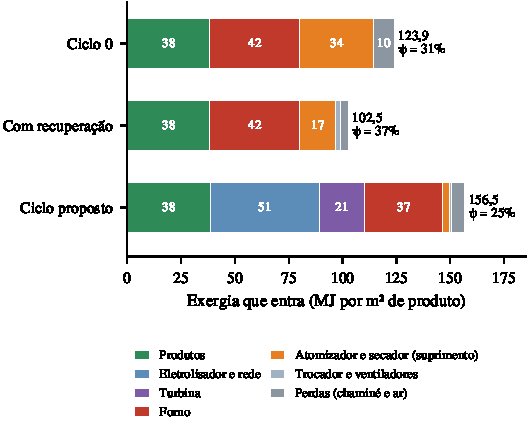
\includegraphics[width=\columnwidth]{figs/fig_exergia_rev.pdf}
\caption{Destino da exergia que entra em cada cenário, por m² de produto: produtos, exergia destruída em cada bloco e perdas; $\psi$ é a eficiência exergética (produtos ÷ entrada). No ciclo proposto, a entrada inclui a eletricidade do campo fotovoltaico.}\label{fig:exergia}
\end{figure}

\begin{table}[!t]
\centering
\caption{Balanço de exergia por m² de produto (MJ)}\label{tab:exergia}
\footnotesize
\begin{tabular}{L{3.55cm}rrr}
\toprule
& \textbf{Ciclo 0} & \textbf{Recup.} & \textbf{Proposto}\\ \midrule
Entra: gás natural & 109,5 & 87,5 & 44,1\\
Entra: eletricidade (rede ou campo) & 14,4 & 15,0 & 112,4\\
Produtos (com o \Ot{} vendido) & 38,4 & 38,4 & 38,5\\
Destruída: rede e eletrolisador & -- & -- & 50,7\\
Destruída: turbina & -- & -- & 21,0\\
Destruída: forno & 41,7 & 41,7 & 36,5\\
Destruída: suprimento do atomizador & 24,3 & 12,9 & 2,2\\
Destruída: suprimento do secador & 10,0 & 3,8 & 1,1\\
Destruída: trocador e ventiladores & -- & 2,4 & 0,6\\
Perdas (chaminés e ar) & 9,6 & 3,4 & 6,0\\
\midrule
Eficiência exergética $\psi$ & 31,0\% & 37,4\% & 24,6\%\\
\bottomrule
\end{tabular}
\end{table}

\textit{Resultados.} A recuperação de calor é a única medida que melhora a eficiência exergética, de 31,0\% para 37,4\% (Tabela~\ref{tab:exergia} e Fig.~\ref{fig:exergia}): ela não muda o forno, mas reduz a destruição no suprimento do atomizador e do secador de 34,3 para 16,7~MJ/m², porque o ar a 150 e 225~°C troca gás natural queimado para produzir gás a 125 e 550~°C. O ganho por MJ recuperado é maior no secador: ali a corrente recuperada já está perto da temperatura de uso, e a destruição cai 62\%, contra 47\% no atomizador. No ciclo proposto, a cascata térmica é a parte mais eficiente: o escape a 500~°C no atomizador e o ar a 225~°C no secador destroem só 3,2~MJ/m². A exergia física das correntes explica a escolha: o escape leva 13,11~MJ/m² (0,402~MJ por MJ sensível) e o ar a 225~°C, 2,60~MJ/m² (0,235); a corrente mais quente vai ao atomizador, que pede gás a 550~°C, e a mais fria ao secador, a 125~°C. Essa comparação usa só correntes de gás calculadas e não depende da exergia retida na peça. Mas a eficiência total, na fronteira ampliada que inclui a eletricidade do campo, cai para 24,6\%, porque a entrada sobe para 156,5~MJ/m²: a rede e o eletrolisador destroem 50,7~MJ/m² e a turbina, 21,0. Esse é o custo termodinâmico do caminho eletricidade → \Ht{} → combustão: cada MJ de calor de \Ht{} no forno pede 1,79~MJ de eletricidade do campo, contra 1,04~MJ de exergia de gás natural, e a eletrólise conserva 56\% da exergia que recebe. O forno continua a maior fonte de destruição dentro da fábrica, como em \cite{ferrer2019,wang2020}; com \Ot, ele destrói 5,1~MJ/m² a menos, porque não aquece o nitrogênio do ar de combustão. A exergia química do \Ot{} é pequena (0,12~MJ/kg; 0,5~MJ/m² no total): o seu valor está em dispensar esse nitrogênio, e não no conteúdo exergético, de modo que uma repartição de custos por exergia daria a ele menos de 1\% do custo da eletrólise. Com o rendimento de 35\%, a turbina destrói 3,0~MJ/m² a menos, mas o eletrolisador destrói 1,7 a mais, e $\psi$ fica praticamente igual.

\textit{Custo da exergia.} Como primeiro passo exergoeconômico, o custo médio da exergia de cada insumo é de US\$~56,2/GJ para o \Ht{} (6,58~US\$/kg ÷ 117,1~MJ/kg), US\$~31,2/GJ para a eletricidade evitada e US\$~17,5/GJ para o gás natural. Cada GJ de exergia levado ao forno como \Ht{} custa 3,2 vezes o do gás, e o forno, que recebe 51~MJ/m² de exergia de \Ht, concentra o custo do ciclo. A turbina é o bloco com dois produtos. Pelo método SPECO \cite{lazzaretto2006}, com o mesmo custo por unidade de exergia para a eletricidade e para o escape, os US\$~13,8 milhões por ano da turbina (capital 1,6, manutenção 0,3, gás natural 8,9, a R\$~3,6537/m³ médios da TG1, e \Ht{} 3,1) se repartem entre 15,00~MJ/m² de eletricidade e 13,11~MJ/m² de escape: US\$~44,8/GJ, ou 0,671~US\$/m² para a eletricidade e 0,587~US\$/m² (47\%) para o escape. A eletricidade da turbina custa assim 0,161~US\$/kWh, cerca de R\$~0,86/kWh, acima dos R\$~0,60/kWh adotados para a rede: é o escape, que troca gás no atomizador, que paga a geração na planta. A aplicação do método a todos os componentes, que exige a tabela de vazões, temperaturas, pressões e composições de todas as correntes e a do forno por zonas, fica para trabalho futuro.

\section{Análise crítica}\label{sec:critica}

\textit{Hipóteses fortes.} A queima de \Ht{} com \Ot{} puro em forno cerâmico não é prática comercial: a chama muito quente, a formação de NO\textsubscript{x} com o ar de processo e o vapor no forno exigiriam estudo próprio. A exergia retida na peça (10\% da entrada) foi medida por \cite{ferrer2019} num forno a gás e aqui é aplicada também ao forno a \Ht, como produto igual nos três cenários; num forno a \Ht{} ela pode ser outra, e a comparação da destruição no forno entre os cenários depende dessa hipótese. Os resultados valem para a indústria de referência do ciclo 0, sem reaproveitamento, cujo consumo foi tomado igual ao de Tijucas (Seção~\ref{sec:dados}). A verificação de temperatura no atomizador (Eq.~\eqref{eq:matmax}) mostrou que somar energia não basta: a divisão do calor recuperado entre as operações é limitada pela massa de gás admissível a 550~°C. A lama de retífica (0,78~kg/m², hipótese) entra só no balanço de massa e não altera a energia.

\textit{Energia e emissões.} A redução de 61\% do \COt{} fóssil custa 26\% mais energia total, 6,4 pontos de eficiência exergética e um campo de 223~ha fora da planta. Ligar o campo e o eletrolisador à rede reduziu o eletrolisador para 43,8~MW, mas torna o hidrogênio renovável apenas por balanço anual e transfere à rede a variação da fotovoltaica. A Lei nº 14.948/2024 não pede coincidência horária, mas a certificação do hidrogênio de baixa emissão depende de regulamento, com análise de ciclo de vida e fronteiras do sistema próprias (arts. 15 a 25) \cite{lei14948}: a compensação anual não garante, por si só, a certificação.

\textit{Carbono.} O projeto não recebe crédito pelo carbono evitado: para empatar, a tonelada teria de valer US\$~562, contra cerca de €~90/t no mercado europeu em novembro de 2026 \cite{yermolenko2026}. No SBCE, o operador que emite mais de 25~mil~t~\COt{}e/ano tem de conciliar todas as suas emissões (art. 30, II, e art. 34 da Lei nº 15.042/2024) \cite{lei15042}; o ciclo 0 emitiria 64,9~mil~t/ano de escopo 1 e o ciclo proposto, com o rendimento do Taurus 60, 26,1~mil~t/ano: o projeto reduz as emissões a conciliar a 40\% das do ciclo 0, mas não tira a fábrica da conciliação: fica 1,1~mil~t/ano acima do limite, sem contar o \COt{} dos carbonatos da massa, que não foi levantado. Com 35\%, ficaria em 23,5~mil~t/ano, abaixo do limite. Nos dois casos, o enquadramento efetivo depende da regulamentação da lei e da contabilização dos carbonatos.

\textit{Economia.} O preço do eletrolisador parte do custo chinês: a engenharia e a obra seguem a proporção chinesa, e os 1.284~US\$/kW em Tijucas ficam abaixo da faixa da IEA para fora da China \cite{iea2025a}; o resultado é otimista nesse item. A tarifa da usina foi tomada igual à das eólicas; uma usina desse porte pode se ligar em tensão mais alta e pagar outra tarifa. O estoque de \Ht{} guarda um dia de consumo (15,7~t, US\$~33,0 milhões), embora só o excedente médio de 2,1~t/dia passe por ele; sem a reserva para paradas longas, o VPL melhora US\$~33 milhões (Tabela~\ref{tab:robustez}). O acerto na CCEE usa o preço médio de cada mês e hora de 2024 e 2025, sem os dias nublados de preço alto, e pode estar subestimado. Os custos que ficaram fora (Seção~\ref{sec:fluxo}) só piorariam o resultado. Separado em duas etapas, o resultado fica mais claro: a recuperação de calor, sozinha, tem VPL de +US\$~41,4 milhões e evita 12,9~mil~t/ano; passar dela ao ciclo proposto custa mais US\$~283,8 milhões de VPL para evitar outras 27,5~mil~t/ano, cerca de 970~US\$/t. O custo médio de 562~US\$/t mistura uma etapa que dá lucro com outra muito cara.

\section{Conclusões}

Numa fábrica de porcelanato de 30.000~m²/dia, 43,43~\MJt/m² saem do forno sem uso. Recuperar esse calor corta 19\% das emissões com equipamentos convencionais, custa cerca de US\$~0,9 milhão (estimativa preliminar), poupa cerca de US\$~4,0 milhões por ano (VPL de +US\$~41 milhões) e é a única medida que melhora a eficiência exergética (de 31\% para 37\%), com mais ganho onde a corrente recuperada está perto da temperatura de uso; por isso deveria ser a primeira medida, e o \Ht{} a segunda, quando o gás ou o carbono encarecerem: da recuperação ao ciclo proposto, cada tonelada evitada custa cerca de 970~US\$. O ciclo com turbina a 30\% de \Ht, cascata térmica e forno a \Ot, com o rendimento de catálogo da turbina orçada, reduz em 61\% o \COt{} fóssil, mas consome 26\% mais energia, tem eficiência exergética de 25\% na fronteira ampliada, por causa da rede e do eletrolisador (50,7~MJ/m²) e da turbina (21,0~MJ/m²), e não tira a fábrica da conciliação do SBCE. Com todos os custos orçados, o VPL é de −US\$~242,4 milhões e o \Ht{} custa US\$~6,58/kg; em nenhuma das 10.000 combinações de hipóteses o projeto se paga com o gás de hoje, e o gás teria de passar de R\$~10,99/m³ para ele se pagar com 90\% de probabilidade. O eletrolisador mínimo, parado só na ponta, é o de menor custo, e cada uso do \Ht{} custa de 614 a 670~US\$/t de \COt{} evitada. Frente aos estudos anteriores, o trabalho mostra, com um modelo verificado e disponível, que a integração térmica é a parte barata e eficiente da descarbonização, e que o custo está no caminho eletricidade → \Ht{} → calor.

\section*{Disponibilidade de dados e código}

O modelo técnico (179 grandezas com fórmula e fonte), o econômico e os scripts da sensibilidade, do Monte Carlo (gerador mulberry32, semente 20261126), da otimização, da análise exergética e das figuras estão em \url{https://github.com/dudxmann/porcelanato-h2-ceramica}. Os dados de processo da Portobello são de uso acadêmico e entram só como os valores agregados citados no texto.

\section*{Agradecimentos}

Os autores agradecem à Portobello pelos dados de processo da unidade de Tijucas, cedidos para uso acadêmico, e ao Prof. Osvaldo J. Venturini pela orientação ao longo da disciplina.

\renewcommand{\refname}{Referências}
\begin{thebibliography}{99}
\setlength{\itemsep}{0pt}\footnotesize
\input{refs_ordenadas_rev.tex}
\end{thebibliography}

\end{document}
